% Standalone render of the Figure 1 architecture diagram for README.md.
% The drawing itself lives in deliverables/d2/report/images/architecture.tikz and is \input here, so the
% README image always follows the report figure. To re-render after the tikz file changes:
%
%   cd docs/images
%   pdflatex -interaction=nonstopmode architecture.tex
%   gs -q -dNOPAUSE -dBATCH -sDEVICE=png16m -dTextAlphaBits=4 -dGraphicsAlphaBits=4 -r240 -sOutputFile=architecture.png architecture.pdf
%   (about 1665 px wide, white background; pdftoppm was not installed on the authoring machine)
%
% Preamble below mirrors deliverables/d2/report/main_d2.tex (fonts, xcolor, tikz + arrows.meta, calc, \code).
\documentclass[border=6pt]{standalone}
\usepackage[utf8]{inputenc}
\usepackage[T5]{fontenc}
\usepackage{lmodern}
\usepackage{xcolor}
\usepackage{tikz}
\usetikzlibrary{arrows.meta,calc}
\newcommand{\code}[1]{\texttt{\detokenize{#1}}}
\begin{document}
% Figure 1 (two-phase architecture: offline ingestion/indexing + online bounded agent loop).
% Drawn at true size, 17.0 cm wide.
% Encoding (Okabe-Ito blue/orange; every class also differs in border style or tag text, so it reads in greyscale):
%   blue fill   = core active component (always on)
%   orange fill = configurable active component with on/off switch (ablated in Section 5)
%   dashed      = implemented in code, disabled in current benchmark runs
%   grey fill   = terminal state of a run
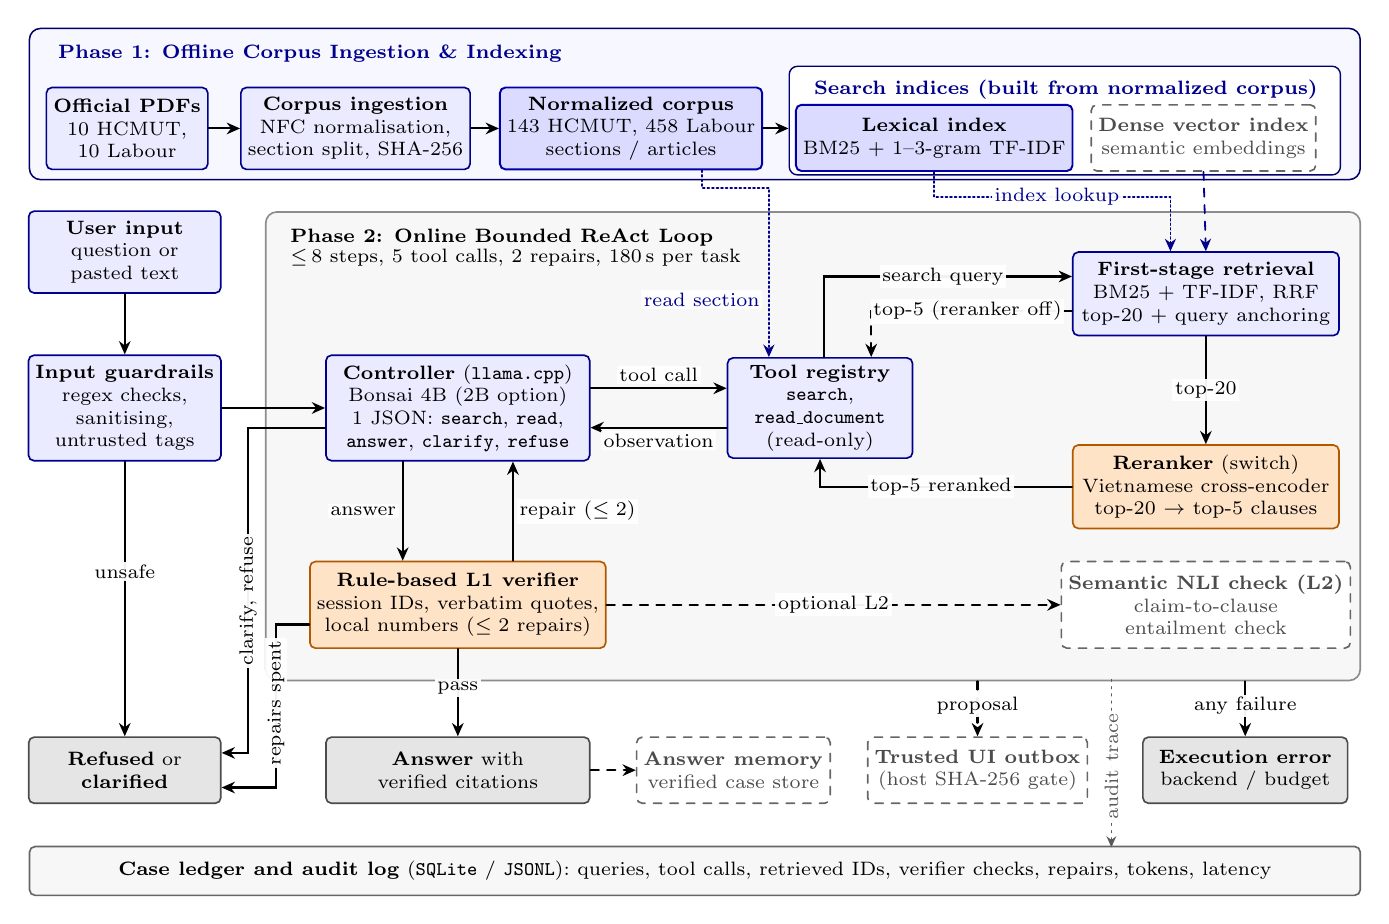
\begin{tikzpicture}[x=1cm,y=1cm,font=\fontsize{7}{8.2}\selectfont,line cap=round,
  box/.style={draw=blue!55!black,fill=blue!8,rounded corners=2pt,align=center,inner sep=2.5pt,minimum height=0.82cm,line width=0.6pt},
  store/.style={box,draw=blue!65!black,fill=blue!14,line width=0.7pt},
  var/.style={box,draw=orange!70!black,fill=orange!22},
  off/.style={box,dashed,draw=black!60,fill=white,text=black!70},
  term/.style={box,draw=black!70,fill=black!10},
  frame/.style={draw=black!45,fill=black!3,rounded corners=4pt,line width=0.6pt},
  pframe/.style={draw=blue!40!black,fill=blue!3,rounded corners=4pt,line width=0.55pt},
  flow/.style={-{Stealth[length=4.8pt,width=4.2pt]},line width=0.75pt},
  dflow/.style={-{Stealth[length=4.5pt,width=4.0pt]},line width=0.65pt,blue!55!black,densely dotted},
  alt/.style={flow,dashed},
  logl/.style={-{Stealth[length=4pt,width=3.5pt]},line width=0.6pt,dotted,black!65},
  lab/.style={font=\fontsize{6.8}{8}\selectfont,inner sep=1.0pt,fill=white,fill opacity=0.94,text opacity=1}]

% =====================================================================
% PHASE 1: OFFLINE INGESTION & INDEXING PIPELINE (TOP BAND)
% =====================================================================
\node[pframe,minimum width=16.9cm,minimum height=1.92cm,anchor=north west] (p1) at (0,10.78) {};
\node[anchor=north west,font=\fontsize{7}{8.2}\selectfont\bfseries,text=blue!55!black] at (0.25,10.68) {Phase 1: Offline Corpus Ingestion \& Indexing};

\node[box,minimum width=2.05cm,minimum height=1.04cm] (pdf) at (1.25,9.50) {\textbf{Official PDFs}\\10 HCMUT,\\10 Labour};
\node[box,minimum width=2.65cm,minimum height=1.04cm] (ing) at (4.15,9.50) {\textbf{Corpus ingestion}\\NFC normalisation,\\section split, SHA-256};
\node[store,minimum width=2.75cm,minimum height=1.04cm] (corp) at (7.65,9.50) {\textbf{Normalized corpus}\\143 HCMUT, 458 Labour\\sections / articles};

% Search indices group built from Normalized corpus
\node[draw=blue!45!black,fill=white,rounded corners=3pt,line width=0.5pt,minimum width=7.00cm,minimum height=1.38cm,anchor=west] (idx) at (9.65,9.60) {};
\node[anchor=north west,font=\fontsize{6.6}{7.8}\selectfont\bfseries,text=blue!55!black] at (9.85,10.24) {Search indices (built from normalized corpus)};
\node[store,minimum width=2.90cm,minimum height=0.84cm] (lex) at (11.50,9.38) {\textbf{Lexical index}\\BM25 + 1--3-gram TF-IDF};
\node[off,minimum width=2.85cm,minimum height=0.84cm] (vec) at (14.92,9.38) {\textbf{Dense vector index}\\semantic embeddings};

\draw[flow] (pdf) -- (ing);
\draw[flow] (ing) -- (corp);
\draw[flow] (corp.east) -- (idx.west |- corp.east);

% =====================================================================
% PHASE 2: ONLINE BOUNDED AGENT & VERIFICATION LOOP (MAIN BAND)
% =====================================================================
\node[frame,minimum width=13.9cm,minimum height=5.95cm,anchor=north west] (fr) at (3.0,8.45) {};
\node[anchor=north west,align=left,font=\fontsize{7}{8.2}\selectfont\bfseries] at (3.2,8.35) {Phase 2: Online Bounded ReAct Loop\\[-1pt]{\normalfont $\le$\,8 steps, 5 tool calls, 2 repairs, 180\,s per task}};

% input column (all x=1.22, width=2.44cm)
\node[box,minimum width=2.44cm,minimum height=1.04cm] (q) at (1.22,7.93) {\textbf{User input}\\question or\\pasted text};
\node[box,minimum width=2.44cm,minimum height=1.34cm] (g) at (1.22,5.95) {\textbf{Input guardrails}\\regex checks,\\sanitising,\\untrusted tags};

% loop body (left col x=5.45 width=3.35cm; mid col x=10.05 width=2.35cm; right col x=14.95 width=3.38cm)
\node[box,minimum width=3.35cm,minimum height=1.34cm] (c) at (5.45,5.95) {\textbf{Controller} (\texttt{llama.cpp})\\Bonsai 4B (2B option)\\1 JSON: \texttt{search}, \texttt{read},\\\texttt{answer}, \texttt{clarify}, \texttt{refuse}};
\node[box,minimum width=2.35cm,minimum height=1.16cm] (t) at (10.05,5.95) {\textbf{Tool registry}\\\texttt{search},\\\texttt{read\_document}\\(read-only)};
\node[box,minimum width=3.38cm,minimum height=1.06cm] (r) at (14.95,7.40) {\textbf{First-stage retrieval}\\BM25 + TF-IDF, RRF\\top-20 + query anchoring};
\node[var,minimum width=3.38cm,minimum height=1.06cm] (rr) at (14.95,4.95) {\textbf{Reranker} (switch)\\Vietnamese cross-encoder\\top-20 $\to$ top-5 clauses};
\node[var,minimum width=3.35cm,minimum height=1.10cm] (v) at (5.45,3.45) {\textbf{Rule-based L1 verifier}\\session IDs, verbatim quotes,\\local numbers ($\le 2$ repairs)};
\node[off,minimum width=3.38cm,minimum height=1.10cm] (l2) at (14.95,3.45) {\textbf{Semantic NLI check (L2)}\\claim-to-clause\\entailment check};

% terminal states and side components (bottom row, all y=1.35, height=0.84cm)
\node[term,minimum width=2.44cm,minimum height=0.84cm] (ref) at (1.22,1.35) {\textbf{Refused} or\\\textbf{clarified}};
\node[term,minimum width=3.35cm,minimum height=0.84cm] (ans) at (5.45,1.35) {\textbf{Answer} with\\verified citations};
\node[off,minimum width=2.45cm,minimum height=0.84cm] (mem) at (8.95,1.35) {\textbf{Answer memory}\\verified case store};
\node[off,minimum width=2.65cm,minimum height=0.84cm] (out) at (12.05,1.35) {\textbf{Trusted UI outbox}\\(host SHA-256 gate)};
\node[term,minimum width=2.60cm,minimum height=0.84cm] (err) at (15.45,1.35) {\textbf{Execution error}\\backend / budget};
\node[box,fill=black!3,draw=black!60,minimum width=16.9cm,minimum height=0.62cm,anchor=south west] (led) at (0,-0.25) {\textbf{Case ledger and audit log} (\texttt{SQLite} / \texttt{JSONL}): queries, tool calls, retrieved IDs, verifier checks, repairs, tokens, latency};

% offline-to-online data connections
\draw[dflow] (lex.south) -- ++(0,-0.32) -| node[lab,pos=0.26]{index lookup} ([xshift=-0.45cm]r.north);
\draw[dflow,dashed] (vec.south) -- (r.north);
\draw[dflow] ([xshift=0.90cm]corp.south) -- ++(0,-0.22) -| node[lab,pos=0.83,left=2pt]{read section} ([xshift=-0.65cm]t.north);

% control flow inside the loop
\draw[flow] (q) -- (g);
\draw[flow] (g) -- (c);
\draw[flow] ([yshift=0.25cm]c.east) -- node[lab,above=1pt]{tool call} ([yshift=0.25cm]t.west);
\draw[flow] ([yshift=-0.25cm]t.west) -- node[lab,below=1pt]{observation} ([yshift=-0.25cm]c.east);
\draw[flow] ([xshift=-0.7cm]c.south) -- node[lab,left=1pt]{answer} ([xshift=-0.7cm]v.north);
\draw[flow] ([xshift=0.7cm]v.north) -- node[lab,right=1pt]{repair ($\le 2$)} ([xshift=0.7cm]c.south);

% search path: query goes out above, results come back below (nested, no crossings)
\draw[flow] ([xshift=0.05cm]t.north) |- node[lab,pos=0.74]{search query} ([yshift=0.22cm]r.west);
\draw[alt] ([yshift=-0.22cm]r.west) -| node[lab,pos=0.26]{top-5 (reranker off)} ([xshift=0.65cm]t.north);
\draw[flow] (r) -- node[lab]{top-20} (rr);
\draw[flow] (rr.west) -| node[lab,pos=0.26]{top-5 reranked} (t.south);
\draw[alt] (v.east) -- node[lab]{optional L2} (l2.west);

% exits
\draw[flow] (g.south) -- node[lab,pos=0.4]{unsafe} (ref.north);
\draw[flow] ([yshift=-0.25cm]c.west) -- ++(-0.98,0) coordinate (cl) |- ([yshift=0.22cm]ref.east);
\node[lab,rotate=90] at (cl |- 0,3.5) {clarify, refuse};
\draw[flow] ([yshift=-0.25cm]v.west) -- ++(-0.42,0) coordinate (rs) |- ([yshift=-0.22cm]ref.east);
\node[lab,rotate=90] at (rs |- 0,2.2) {repairs spent};
\draw[flow] (v.south) -- node[lab,pos=0.45]{pass} (ans.north);
\draw[alt] (ans.east) -- (mem.west);
\draw[alt] (fr.south -| out) -- node[lab,pos=0.45]{proposal} (out.north);
\draw[flow] (fr.south -| err) -- node[lab,pos=0.45]{any failure} (err.north);
\draw[logl] (13.75,2.50) -- node[lab,rotate=90,pos=0.52]{audit trace} (13.75,0.37);
\end{tikzpicture}

\end{document}
